%% Diagram of systems development life cycle
%%
%% Base TikZ taken from <http://www.texample.net/tikz/examples/circular-arrows-text/>.
%%
%% See also: sdlc-preamble.tex
\usetikzlibrary{decorations.text}
\newcommand*{\mytextstyle}{\sffamily\normalsize\bfseries\color{black!85}}
\newcommand{\arcarrow}[8]{%
% inner radius, middle radius, outer radius, start angle,
% end angle, tip protusion angle, options, text
  \pgfmathsetmacro{\rin}{#1}
  \pgfmathsetmacro{\rmid}{#2}
  \pgfmathsetmacro{\rout}{#3}
  \pgfmathsetmacro{\astart}{#4}
  \pgfmathsetmacro{\aend}{#5}
  \pgfmathsetmacro{\atip}{#6}
  \fill[#7] (\astart:\rin) arc (\astart:\aend:\rin)
       -- (\aend+\atip:\rmid) -- (\aend:\rout) arc (\aend:\astart:\rout)
       -- (\astart+\atip:\rmid) -- cycle;
  \path[font = \sffamily, decoration = {text along path, text = {|\mytextstyle|#8},
    text align = {align = center}, raise = -0.5ex}, decorate]
    (\astart+\atip:\rmid) arc (\astart+\atip:\aend+\atip:\rmid);
}

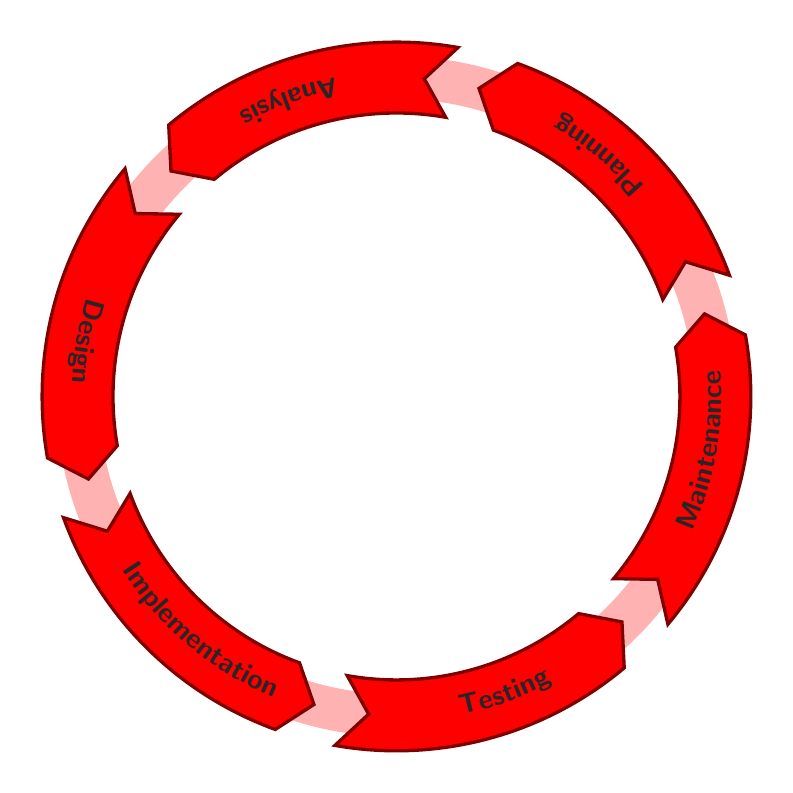
\begin{tikzpicture}[scale=0.9]
  \fill[even odd rule,red!30] circle (4.8) circle (4.2);
  \foreach \x/\text in {0/Planning,1/Analysis,2/Design,3/Implementation,4/Testing,5/Maintenance} {
    \arcarrow{4}{4.5}{5}{\x*60+20}{\x*60+70}{5}{red,draw = red!50!black, very thick}{\text}
  }
\end{tikzpicture}
